\documentclass[a4paper]{article}

\usepackage{amsmath}
\usepackage{amssymb}
\usepackage{graphicx}
\usepackage{float}
\usepackage[margin=1in]{geometry}
\usepackage{titlesec}
\usepackage{listings}
\usepackage{color}
\graphicspath{ {Images/} }
\renewcommand{\baselinestretch}{1.2}
\setlength\parindent{0pt}
\setlength{\parskip}{\baselineskip}
% ------------------- Matlab Converter to LATEX ------------------- %
%red, green, blue, yellow, cyan, magenta, black, white
\definecolor{mygreen}{RGB}{28,172,0} % color values Red, Green, Blue
\definecolor{mylilas}{RGB}{170,55,241}
\lstset{language=Matlab,%
%basicstyle=\color{red},
breaklines=true,%
morekeywords={matlab2tikz},
keywordstyle=\color{blue},%
morekeywords=[2]{1}, keywordstyle=[2]{\color{black}},
identifierstyle=\color{black},%
stringstyle=\color{mylilas},
commentstyle=\color{mygreen},%
showstringspaces=false,%without this there will be a symbol in the places where there is a space
    %numbers=left,%
    %numberstyle={\tiny \color{black}},% size of the numbers
    %numbersep=9pt, % this defines how far the numbers are from the text
emph=[1]{for,end,break},emphstyle=[1]\color{blue}, %some words to emphasise
    %emph=[2]{word1,word2}, emphstyle=[2]{style},    
}
% This will add the units to the nomenclature
% ------------------- Matlab Converter to LATEX ------------------- %
\newcommand{\nomunit}[1]{%
\renewcommand{\nomentryend}{\hspace*{\fill}#1}}
%----------------------------------------------
 
\begin{document} 

\begin{figure}[H]
\centering
\includegraphics[scale=0.8]{LOGO}
\end{figure} 

\begin{center}\begin{Large}

Tom Smadar 203374061

Daniel Engelsman 300546173
\end{Large} \end{center}


% --------------- Section 2 --------------- %
\section{Repeat Lab 3}

\subsection{Matlab Code + Explanations}

\lstinputlisting{Q1.m}
\newpage

\subsection{Results - Fixed Images}
Chosen Image where both landmarks are clearly visible, and then launching the algorithm :
\begin{figure}[H]
\centering
\includegraphics[scale=0.5]{1_a}
\caption{Image $\#$ 96} 
\end{figure}

We can see that the projected points (marked blue) are quite close to the manually selected ones (marked red). There is a “height” difference that might pertain to the camera calibration matrix.

\begin{figure}[H]
\centering
\includegraphics[scale=0.5]{1_b}
\caption{Image $\#$ 96 after Projected crosses }
\end{figure}

The Re-projection error for the landmarks :
\begin{figure}[H]
\centering
\includegraphics[scale=0.4]{1_c}
\caption{Error Table} 
\end{figure}
\newpage

% --------------- Section 2 --------------- %
\section{Image correspondence for the entire database}

\subsection{Landmarks Visibility}

\begin{figure}[H]
\centering
\includegraphics[scale=0.5]{2_a}
\caption{Landmarks Visibility (“1” for visible and “0”) from Robot Position} 
\end{figure}

\subsection{Graph Presentation}

\lstinputlisting{Q2.m}

\begin{figure}[H]
\centering
\includegraphics[scale=0.45]{2_b}
\caption{ Landmarks Correspondence to Robot Position } 
\end{figure}
\newpage

% --------------- Section 3 --------------- %
\section{Auxiliary Transformation Matrix}
\lstinputlisting{GetTranslationMat.m}

\textbf{Notes : }\begin{flushleft}
$\bullet$ the mo-cap is turned by +90.6 $^{\circ}$ around zaxis, in reference to the
robot’s coordinate system. \\

$\bullet$ The function uses few global variables for simplicity reasons. \end{flushleft}
\newpage 

% --------------- Section 4 --------------- %
\section{Triangulate a landmark}
\subsection*{Matlab Code}

\lstinputlisting{Q4_a.m}

\subsection{Choose 3 different images in which L2 visible}
\begin{figure}[H]
\centering
\includegraphics[scale=0.4]{4_set}
\caption{ Set of Images [1 32 96] } 
\end{figure}

\subsection{Manual Extraction}
\begin{figure}[H]
\centering
\includegraphics[scale=0.6]{4_a}
\caption{ Obtained Pixels of the manual Extraction } 
\end{figure} \newpage


\subsection{Reconstruction at both Methods }
\subsection*{Matlab Code}

\lstinputlisting{Q4_cd.m}

\textbf{Note : }
\begin{flushleft}
$\bullet$ The code refers to both methods (odometry / mo-cap)  depends on the flag value.

$\bullet$ The u and v pixels as seen above, have been extracted from Pix1, Pix2, Pix3 matrix arrays. \end{flushleft} \newpage

\subsection{ 3D Presentation of Triangulation points }
\lstinputlisting{Q4_e.m}

\begin{figure}[H]
\centering
\includegraphics[scale=0.52]{4_Plot_Show}
\caption{ 3D Scatter of Triangulation points after Reconstruction } 
\end{figure}

\subsection{ 3D location error of L2 for both Methods }

\begin{figure}[H]
\centering
\includegraphics[scale=0.6]{4_calculation}
\caption{ Absolute Error between Reconstructed Landmarks to Ground Truth } 
\end{figure}
\newpage


% --------------- Section 5 --------------- %
\section{The importance of diversity}

\subsection{ 3D location error of L2 for both Methods }

\lstinputlisting{Q5_a.m}

\textbf{Note : }
\begin{flushleft}
$\bullet$ As requested, frames increase monotonously along time.\\
$\bullet$ After first execution, pixels values were saved aside.
\end{flushleft}

\subsection{ Impact of Poses' Variety }
\lstinputlisting{Q_latex_5_b.m}
\newpage

In this section we're requested to present a correlation between variety in poses and and 3D triangulation error. In order to do so we need to choose a compatible segment that fulfils 3 conditions : 

1. \textbf{Line Of Sight : } The robot "sees" Landmark 2 along the segment (\textbf{Figure 4}).

2. \textbf{Motion : } Triangulation occurs while the robot moves along route.

3. \textbf{Variance :} The error differs between the images in the segment, and is not constant.

The chosen segment that satisfies these 3 requirement, is the marked \textbf{Window of opportunity } : 

\begin{figure}[H]
\centering
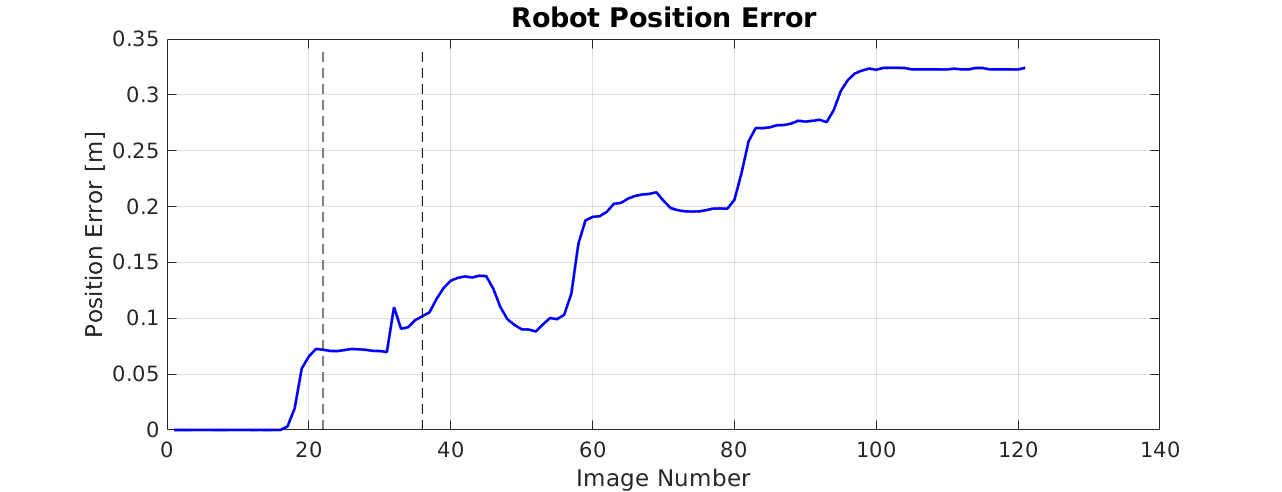
\includegraphics[scale=0.48]{Rob_Pose_Err}
\caption{ Images 22:36 domain} 
\end{figure} 

And now we'll calculate the 3D triangulation error vs. the Weighted Normalized Difference :

\begin{figure}[H]
\centering
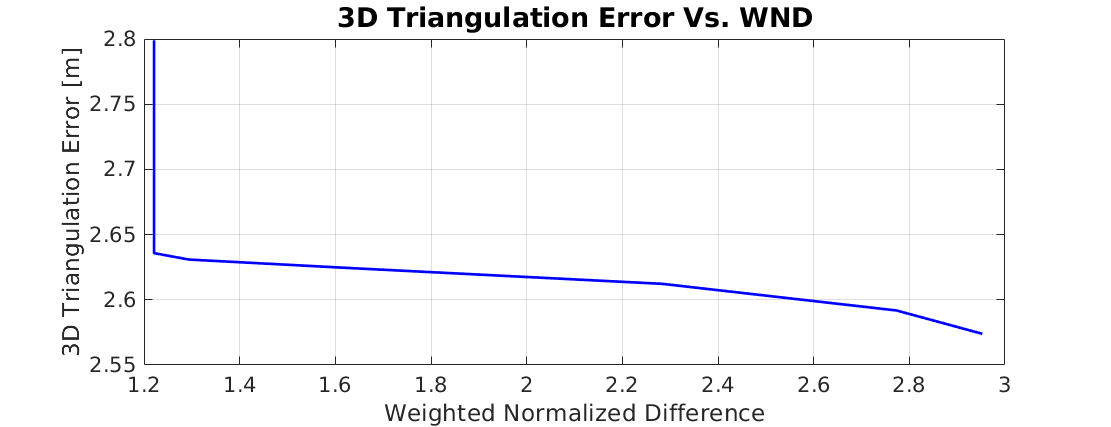
\includegraphics[scale=0.56]{3DvsWND}
\caption{3D Triangulation Vs WND} 
\end{figure} 

One can see the 3D error declination as function of the robot progression. However, the sharp asymptote at the beginning is explained by the robot's sharp twist while taking the 1st picture.
\newpage

\subsection{ Results Presentation }
\lstinputlisting{Q5_c.m}

Hereby presented a graph showing the the results :
\begin{figure}[H]
\centering
\includegraphics[scale=0.6]{5_c}
\caption{Results Presentation} 
\end{figure} 
\newpage

\subsection{ Used Frames }
\begin{figure}[H]
\centering
\includegraphics[scale=0.423]{set_1}
\caption{1st Set of Images [5 18 20]} 
\end{figure} 

\begin{figure}[H]
\centering
\includegraphics[scale=0.4]{set_2}
\caption{2nd Set of Images 24 26 27]} 
\end{figure} 

\begin{figure}[H]
\centering
\includegraphics[scale=0.4]{set_3}
\caption{3rd Set of Images [30 32 34]} 
\end{figure} 

\begin{figure}[H]
\centering
\includegraphics[scale=0.4]{set_4}
\caption{4th Set of Images [96 100 115]} 
\end{figure} 


\end{document}
